%Version 3 October 2023
% See section 11 of the User Manual for version history
%
%%%%%%%%%%%%%%%%%%%%%%%%%%%%%%%%%%%%%%%%%%%%%%%%%%%%%%%%%%%%%%%%%%%%%%
%%                                                                 %%
%% Please do not use \input{...} to include other tex files.       %%
%% Submit your LaTeX manuscript as one .tex document.              %%
%%                                                                 %%
%% All additional figures and files should be attached             %%
%% separately and not embedded in the \TeX\ document itself.       %%
%%                                                                 %%
%%%%%%%%%%%%%%%%%%%%%%%%%%%%%%%%%%%%%%%%%%%%%%%%%%%%%%%%%%%%%%%%%%%%%

%%\documentclass[referee,sn-basic]{sn-jnl}% referee option is meant for double line spacing

%%=======================================================%%
%% to print line numbers in the margin use lineno option %%
%%=======================================================%%

%%\documentclass[lineno,sn-basic]{sn-jnl}% Basic Springer Nature Reference Style/Chemistry Reference Style

%%======================================================%%
%% to compile with pdflatex/xelatex use pdflatex option %%
%%======================================================%%

%%\documentclass[pdflatex,sn-basic]{sn-jnl}% Basic Springer Nature Reference Style/Chemistry Reference Style


%%Note: the following reference styles support Namedate and Numbered referencing. By default the style follows the most common style. To switch between the options you can add or remove “Numbered” in the optional parenthesis. 
%%The option is available for: sn-basic.bst, sn-vancouver.bst, sn-chicago.bst%  
 
%%\documentclass[sn-nature]{sn-jnl}% Style for submissions to Nature Portfolio journals
%%\documentclass[sn-basic]{sn-jnl}% Basic Springer Nature Reference Style/Chemistry Reference Style
\documentclass[sn-mathphys-num]{sn-jnl}% Math and Physical Sciences Numbered Reference Style 
%%\documentclass[sn-mathphys-ay]{sn-jnl}% Math and Physical Sciences Author Year Reference Style
%%\documentclass[sn-aps]{sn-jnl}% American Physical Society (APS) Reference Style
%%\documentclass[sn-vancouver,Numbered]{sn-jnl}% Vancouver Reference Style
%%\documentclass[sn-apa]{sn-jnl}% APA Reference Style 
%%\documentclass[sn-chicago]{sn-jnl}% Chicago-based Humanities Reference Style

%%%% Standard Packages
%%<additional latex packages if required can be included here>

\usepackage{graphicx}%
\usepackage{multirow}%
\usepackage{amsmath,amssymb,amsfonts}%
\usepackage{amsthm}%
\usepackage{mathrsfs}%
\usepackage[title]{appendix}%
\usepackage{xcolor}%
\usepackage{textcomp}%
\usepackage{manyfoot}%
\usepackage{booktabs}%
\usepackage{algorithm}%
\usepackage{algorithmicx}%
\usepackage{algpseudocode}%
\usepackage{listings}%
\usepackage{graphicx}
\usepackage{subcaption}
\usepackage{dirtree}

%%%%

%%%%%=============================================================================%%%%
%%%%  Remarks: This template is provided to aid authors with the preparation
%%%%  of original research articles intended for submission to journals published 
%%%%  by Springer Nature. The guidance has been prepared in partnership with 
%%%%  production teams to conform to Springer Nature technical requirements. 
%%%%  Editorial and presentation requirements differ among journal portfolios and 
%%%%  research disciplines. You may find sections in this template are irrelevant 
%%%%  to your work and are empowered to omit any such section if allowed by the 
%%%%  journal you intend to submit to. The submission guidelines and policies 
%%%%  of the journal take precedence. A detailed User Manual is available in the 
%%%%  template package for technical guidance.
%%%%%=============================================================================%%%%

%% as per the requirement new theorem styles can be included as shown below
\theoremstyle{thmstyleone}%
\newtheorem{theorem}{Theorem}%  meant for continuous numbers
%%\newtheorem{theorem}{Theorem}[section]% meant for sectionwise numbers
%% optional argument [theorem] produces theorem numbering sequence instead of independent numbers for Proposition
\newtheorem{proposition}[theorem]{Proposition}% 
%%\newtheorem{proposition}{Proposition}% to get separate numbers for theorem and proposition etc.

\theoremstyle{thmstyletwo}%
\newtheorem{example}{Example}%
\newtheorem{remark}{Remark}%

\theoremstyle{thmstylethree}%
\newtheorem{definition}{Definition}%

\raggedbottom
%%\unnumbered% uncomment this for unnumbered level heads

\begin{document}

\title[Article Title]{Webapp for Automated Visualization: Matplotlib Plotting for NBA Shooting Stats, Heatmaps, and More}

%%=============================================================%%
%% GivenName	-> \fnm{Joergen W.}
%% Particle	-> \spfx{van der} -> surname prefix
%% FamilyName	-> \sur{Ploeg}
%% Suffix	-> \sfx{IV}
%% \author*[1,2]{\fnm{Joergen W.} \spfx{van der} \sur{Ploeg} 
%%  \sfx{IV}}\email{iauthor@gmail.com}
%%=============================================================%%

\author{\fnm{Emre} \sur{Bayazitoglu}}\email{emre.bayazitoglu@students.uni-freiburg.de}
\affil{\orgdiv{Albert Ludwig University of Freiburg}, \orgaddress{\city{Freiburg}, \country{Germany}}}


%%==================================%%
%% Sample for unstructured abstract %%
%%==================================%%

\abstract{\href{https://www.stats.nba.com}{stats.nba.com} provides a wealth of statistics each season, including data on every player's shooting positions per game. To enhance the visualization of these shooting positions' x- and y-coordinates, I developed a shooting position map using Matplotlib, which plots markings on a pre-drawn basketball court. Motivated by my passion for mathematics and extensive experience with Matplotlib, I also incorporated various mathematical and illustrative plots into this project, such as trigonometric functions, simple functions dependent on one variable, bar charts, and pie charts.

This report offers a review of my experiences, outcomes, and the technologies utilized in my final project for the "Missing Semester" course. Additionally, it provides insights into code examples and methodologies employed in the development and sharing of the final software.

For access to the code and detailed setup instructions, please visit the \href{https://github.com/freiburg-missing-semester-course/project-Emredinho61}{GitHub repository of this project}.
}

\keywords{Vue.js, Python, Flask, Docker, Matplotlib, automated plotting}

%%\pacs[JEL Classification]{D8, H51}

%%\pacs[MSC Classification]{35A01, 65L10, 65L12, 65L20, 65L70}

\maketitle

\section{Introduction}\label{sec1}

The game of basketball is multifaceted, making it crucial to visualize data for analyzing individual players or teams each season. Over the past 20 years, the NBA has collected detailed data to facilitate analysis, with datasets stored in CSV files. To enable data communication, I developed a Python script to transfer this data into a database managed by PySQLite. This database serves as the foundation for a faster and more efficient data retrieval process. Using this database, users can select specific players for each season via a Vue.js frontend. Following user input, they can choose to display \textit{made shots} or \textit{missed shots} as options, which are then analyzed using a Matplotlib Python script. This generates plots that users can utilize for basketball player analysis. All in all, a variety of technologies are employed to automate the process of generating meaningful and customizable plots.

For users that are not interested in basketball, the web app also offers options to plot mathematical functions and charts. These features are accessible through the frontend, where users fill out a form. Upon form submission, the automation starts, making-use of useful Python libraries and frameworks like Flask, a web framework used for communication between the frontend and backend, and NumPy for evaluating mathematical functions inputted by the user.

This report is structured to guide users through the Matplotlib scripts, starting from the frontend via the interface between the frontend and backend. Finally, the process for dockerizing the software is explained.

 

\section{Methodology}\label{sec2}

The project requirements were two fusion two topics from the "Missing Semester" lecture, and I chose the ones that interested me the most: plotting with Matplotlib and automation. Additionally, to facilitate project sharing, I used Docker with Dockerfiles and a \textit{docker-compose.yml} configuration.

The idea came when I discovered the vast dataset provided by \href{https://www.stats.nba.com}{stats.nba.com}, so I decided to create a tool that plots shooting maps for NBA players across different seasons. To achieve this, I began by designing a user-friendly webpage using Vue.js and PrimeVue for the frontend and Flask for handling requests between the frontend and backend.

Having established the frontend-backend interface, I proceeded to develop the backend infrastructure. This included developing a Python script to initialize a database from a CSV file and a Matplotlib script for generating the shooting maps. Recognizing the central role of the database in NBA plotting, priority was set to its creation at the beginning of the dockerization.

Following the frontend and backend design, I focused on ensuring all dependencies were met. To ensure this, I created Dockerfiles for both the frontend and backend, composing them through a \textit{docker-compose.yml} configuration. This approach simplifies dependency management and facilitates project deployment for users.

\section{Automation: Vue.js Frontend and Python Backend}\label{sec3}

Several technologies work together to automate the process of data management, processing, and visualization in the project:

\begin{itemize}
    \item \textbf{Graphical User Interface (GUI):} The GUI runs on a local host and provides a user-friendly interface for interaction. It allows users to input data and visualize results conveniently.
    \item \textbf{Flask Web Server:} Flask is a lightweight web framework for Python \cite{flaskdocu}, used in this project to handle HTTP requests between the frontend and backend.
    \item \textbf{PySQLite-managed Database:} PySQLite is a Python library that provides an interface for interacting with SQLite databases. In this project, it manages the database operations, such as data storage, retrieval, and manipulation. \cite{pysqlitedocu}
\end{itemize}

\subsection{Vue.js Frontend}\label{subsec2}

Once the project is set up successfully, the user can refer to the \href{http://localhost:8080}{GUI} to interact with the software. The software is structured with a panel menu in which the user can choose between several options:

\bigskip
\begin{itemize}
    \item NBA shooting map
    \item simple plotting
    \item bar charts
    \item pie charts
    \item trigonometric functions.
\end{itemize}
\bigskip

The design of the webapp is intended to be intuitive and easy to use. The user simply needs to fill out the forms and is provided with the corresponding plots. In general, communication is implemented using axios. Once a form is filled out, a POST method is executed to provide the backend with the user inputs and receive, most commonly, a plot as a response. The communication is being maintained by an proxy, which was implemented like this:
\bigskip
\begin{verbatim}
const { defineConfig } = require("@vue/cli-service");
module.exports = defineConfig({
  transpileDependencies: true,
  devServer: {
    proxy: {
      "/api": {
        target: "http://172.18.0.2:5000",
        pathRewrite: { "^/api": "" },
      },
    },
  },
});
\end{verbatim}

Since the GUI and the backend web server are not running on the same host (they run in different container), I needed to proxy API requests to the API server. [3]

\begin{itemize}
    \item \texttt{const \{ defineConfig \} = require("@vue/cli-service");}: This line imports the \texttt{defineConfig} function from the \texttt{@vue/cli-service} package.
    
    \item \texttt{transpileDependencies: true}: This configuration option tells Vue CLI to transpile dependencies using Babel \cite{vuecli}. When set to \texttt{true}, all dependencies in the \texttt{node\_modules} directory will be transpiled to ensure compatibility with older browsers \cite{vuecli}.
    
    \item \texttt{devServer}: This section configures the development server options. Which are:
    \begin{itemize}
    \item \texttt{proxy}: Used to forward requests from the used axios methods in the web app to the matching Flask routes. 
    
    \item \texttt{"/api"}: This line specifies the prefix of the requests that should be proxied eg.:

    \begin{verbatim}
    axios.post("/api/postBar", data) \\ send data to the speciefied  
                                      \\ prefix "/api/postBar"
    .then((response) => {
        console.log(respone) \\ log the response
    }).catch((error) => {
        console.log(error);  \\ log possible errors
    })
    \end{verbatim}
    
    \item \texttt{target: "http://172.18.0.2:5000"}: This line specifies the target URL to which requests matching the specified prefix should be forwarded. In this case, requests starting with \texttt{/api} will be forwarded to \texttt{http://172.18.0.2:5000}. Which is the static IP of the docker container.
    
    \item \texttt{pathRewrite: \{ "\^/api": "" \}}: Finally, the \texttt{/api} prefix is removed before sending the request to the Flask-route.
    \end{itemize}
\end{itemize}

Overall, this configuration file sets up a development server for a Vue.js project and configures it to proxy requests to a backend server running at \url{http://172.18.0.2:5000} which is the static ip of the docker container in which the Flask backend server runs.

\subsubsection{NBA Shooting Map}\label{subsubsec1}

The NBA shooting map option features a drop-down component allowing users to select an NBA season ranging from 2004 to 2023. Due to faulty data within the datasets, seasons 2020, 2021, and 2022 are excluded. Additionally, the interface offers two sets of radio buttons. The first set enables users to toggle between viewing options, including a \textit{heat map} or a \textit{position marking map}. The second set provides users with the choice between displaying a plot for \textit{made shots} or \textit{missed shots}.

To enhance usability and organization, the drop-down component for player selection is structured to first prompt users to choose a team before presenting a list of available players. This was realized using the cascade-select component of PrimeVue's component library.


\subsubsection{Simple Plotting}\label{subsubsec2}

The simple plotting option contains of six input fields. The first input field requires users to input a function in a notation interpretable by Python. For example, $x^2$ should be entered as \textit{x**2}. This notation ensures compatibility with Python's syntax for function evaluation. Following the function input, users specify the x-range of the plot using the start and stop input fields. These parameters define the range over which the function will be plotted. Users may use the remaining three input fields to label the x- and y-axes and to assign a title to the plot.

\subsubsection{Bar Charts and Pie Charts}\label{subsubsec3}

The bar chart and pie chart options feature input fields and a table for enhanced customization and data presentation. For the bar chart option, users encounter three input fields for axis and plot labeling. These fields enable users to specify labels for the x-axis, y-axis, and the plot itself, ensuring clear and informative visualizations. Furthermore, the pie chart option includes a single input field for labeling the plot, as pie charts do not have axes like bar charts.

The table structure for both options is organized as depicted in Table \ref{tab:functionality}:

\bigskip
\begin{table}[h]
\centering
\begin{tabular}{|l|p{65mm}|p{35mm}|}
\hline
\textbf{Column} & \textbf{Functionality} & \textbf{Changable in Edit Mode?} \\ \hline
\textbf{ID}    & displays the row number. & No. \\ \hline
\textbf{Name}     & displays the label of the bar or slice. & Yes. \\ \hline
\textbf{Value}     & displays the "height" of the bar chart/portion of the slice of the pie chart (all values must sum up to 100 for the pie chart). & Yes.\\ \hline
\textbf{Color}     & the user can select a color for the corresponding bar or slice. & Yes. A color picker appears. \\ \hline
\end{tabular}
\caption{Functionality of table columns for bar/pie chart}
\label{tab:functionality}
\end{table}
\bigskip

Every row contains a button with a stylus as a label. Once the user clicks on that stylus, the table changes into edit mode, which means that the user can change the row elements.

\subsubsection{Trigonometric Funtions}\label{subsubsec4}

In the trigonometric plotting option, users can plot trigonometric functions with customizable parameters. This option presents seven input fields and one set of radio buttons to define the mode, supporting sine, cosine, and tangent functions. Upon selecting this option, users are prompted to specify a title for the plot. Similar to the simple plotting option, users define the start and stop values for the plot range. The remaining input fields are labeled as \textit{a}, \textit{b}, \textit{c}, and \textit{d}. While these labels may seem imprecise, they correspond to parameters in the following equation:
\bigskip
\[ f(x) = a \times \text{sin}(b \times x + c) + d \]


\begin{itemize}
    \item \textit{a} denotes the amplitude, controlling the vertical stretching or compression of the function \cite{mathisfun}.
    \item \textit{b} denotes the period, representing the horizontal length of one cycle of the function \cite{mathisfun}.
    \item \textit{c} denotes the phase shift, determining the horizontal displacement of the function \cite{mathisfun}.
    \item \textit{d} denotes the vertical shift, indicating the vertical displacement of the function \cite{mathisfun}.
\end{itemize}

These parameters allow users to customize the shape and behavior of the plotted trigonometric function according to their preferences.


\subsection{Python Backend}\label{subsubsec2}

The backend is divided into three individual but yet dependent systems.
\bigskip
\begin{itemize}
    \item Flask app to handle incoming requests from the backend
    \item PySQLite script to create and manage databases
    \item Matplotlib script to generate the plots.
\end{itemize}
\bigskip
The Flask and PySQLite scripts are covered in this section, while the Matplotlib scripts are covered in their own sections.

\subsubsection{Flask App}\label{subsubsubsec1}

The Flask application provides routes to handle various plotting functionalities. For NBA shooting statistics visualization, I created a dedicated route \textit{postPlotNBA} to process user requests, extract relevant data based on user inputs (such as selected player, season, and shot type - \textit{missed shots} or \textit{made shots}), and generate corresponding plots using Matplotlib. Similar routes were implemented for trigonometric function plots \textit{postTrig}, simple function plots \textit{postSimplePlot}, bar charts \textit{postBar}, and pie charts \textit{postPie}. The Flask application script calls the instances of the plotting classes, which are covered in the \hyperref[sec4]{Matplotlib} section. The workflow here is as follows:

\bigskip
\begin{enumerate}
    \item Receive the HTTP-request from the frontend.
    \item Pass the data to the instances of the plotter classes.
    \item Receive the plots from the instances.
    \item Respond to the HTTP-requests with the plots
\end{enumerate}
\bigskip


\subsubsection{PySQLite}\label{subsubsubsec2}

The script that initially sets up the local database uses PySQLite. It is a script that has a simple purpose: create and fill a datatable. The workflow is as follows:
\begin{enumerate}
    \item create an empty database
    \item connect to that database
    \item create a datatable \textit{nbashotsperplayer}, using an SQL query
    \begin{verbatim}
    "CREATE TABLE nbashotsperplayer (SEASON_1 int,
    TEAM_ID int, TEAM_NAME text, PLAYER_ID int,
    PLAYER_NAME text, EVENT_TYPE text, SHOT_MADE text,
    LOC_X double, LOC_Y double);"
\end{verbatim}
    \item open and read the CSV file, extract the columns needed, and insert them into the datatable \textit{nbashotsperplayer}.
\begin{verbatim}
    "INSERT INTO nbashotsperplayer (SEASON_1, TEAM_ID,
    TEAM_NAME, PLAYER_ID, PLAYER_NAME, EVENT_TYPE, SHOT_MADE,
    LOC_X, LOC_Y) VALUES (?, ?, ?, ?, ?, ?, ?, ?, ?);"
\end{verbatim}
\end{enumerate}

\section{Matplotlib}\label{sec4}

The Matplotlib section of the project consists of various classes, each dedicated to a specific type of plot. Instances of these classes are called within the respective routes of the Flask application to handle plot generation based on user requests. The functionality of each class is elaborated upon in the corresponding subsections.

\subsection{Simple Plots Depending on One x}\label{subsec1}

This \textit{SimplePlot} class is designed to create and save simple plots based on user-defined equations that depend on one variable: x. The constructor initializes the instance with parameters representing the equation, start and stop values for the x-axis, x and y-axis labels, and the plot title.
A method within this class generates the plot based on the provided equation and saves it as a PNG image.
First, the method generates an array of evenly spaced numbers (for x) between the start and stop values. When evaluating the provided equation string, NumPy's eval function comes in handy to calculate the corresponding y-values. The calculated points from the function are then projected onto the coordinate system. Finally, a little styling is done to improve the appearance.

\subsection{Trigonometric Functions}\label{subsec2}
Using the provided parameters - amplitude \textit{a}, frequency \textit{b}, phase shift \textit{c}, and vertical shift \textit{d} - the method constructs the function and plots it over a specified range of x-values. The resulting plot is saved as a PNG image with the specified title. NumPy provides all three trigonometric functions as methods in the library. All I needed to do was provide the user-specified values. So the implementation of this was rather easy.

\subsection{Pie Charts and Bar Charts}\label{subsec3}

This class uses the provided parameters, such as the names of each slice with corresponding values and customizable colors. Upon instantiation, the class constructs the pie chart, ensuring each slice represents its proportion of the whole. Afterwards, to enhance readability, annotations to display percentage values within each segment were included. The resulting plot is equipped with the user-inputted title and legend.

\subsection{NBA Shooting}\label{subsec4}
The biggest effort in plotting was put into the NBA shooting maps. The NBA shooting heat and marking maps use a Matplotlib-drawn basketball half-court and map the x- and y-coordinates of the selected players shot on the half-court. The half-court borders are represented by a rectangle. The three-point line is a composition of two straight lines combined with a semicircle. In this three-point box, there is the hoop, which is represented by a circle and a straight line; a circle, which outlines the free-throw line; and finally, the restricted zone, which is also a rectangle. The x-values for the half-court range from -250 to 250, where the origin is the center of the hoop. The y values range from -47.5 to 422.5. Since the x- and y-coordinates of the dataset only range for x from -30 to 30 and for y from 0 to 40, I had to scale the coordinates such that they fit into the half-court properly. Depending on whether the heatmap represents \textit{made shots} or \textit{missed shots}, the title of the plot is dynamically adjusted to reflect the corresponding data.

\subsubsection{Marking Map}\label{subsubsec1}
The marking map uses red crosses if the \textit{missed hots} option is selected in the frontend and green circles if the \textit{made shots} option is selected. After the scaling happens, the points are mapped on the basketball court.

\subsubsection{Heat Map}\label{subsubsec2}
I have created a heatmap plot using the Seaborn library, which depicts the distribution of the data points on a basketball court. The heatmap is customized with a specific colormap style ("YlOrRd\_r") to highlight variations in density. Additionally, the x and y limits are set to ensure the entire half-court is visible.

\section{Docker}\label{sec5}
In order to setup the project locally, the user has to have Docker and Docker Compose installed. In this project, Docker is used to make the setup as easy as possible for the user.
The project setup consists of including the CSV file with the data of the shooting positions into a project folder and then running the command:
\bigskip
\begin{verbatim}
    docker-compose up
\end{verbatim}
\bigskip
in the root folder of the \href{https://github.com/freiburg-missing-semester-course/project-Emredinho61}{repository}.

In the Git repository of this project, there are two Dockerfiles, which are composed using a \textit{docker-compose.yml} configuration. The Dockerfiles set up the environment for the frontend and the backend. For the backend, all the dependencies are installed using \textit{pip}, which is the package installer for Python. In the Dockerfile, the dependencies are installed into the environment like this:

\bigskip
\begin{verbatim}
    RUN python3 -m pip install <package>
\end{verbatim}
\bigskip

The image that is used for the environment is the Python 3.11 image. After installing the dependencies, the backend folder, which contains all the Python scripts, is copied into the Docker container and then executed.
The approach for the frontend is similar. On the frontend, the dependencies are installed using \textit{npm}, which is the package installer specialized for Javascript environments. All the dependencies are specified in the \textit{package.json} and are simply installed using:

\bigskip
\begin{verbatim}
    RUN npm install
\end{verbatim}
\bigskip
Yet again, the folder containing the frontend code is copied into the container. The frontend is then run and served on local host with port 8080 using the command:

\bigskip
\begin{verbatim}
    CMD["npm", "run", "serve"]
\end{verbatim}
\bigskip

The \textit{docker-compose.yml} configuration is then executing the frontend and backend services. Here, the ports of the container are mapped to the ports of the host machine for both services.

\section{Results}\label{sec6}

After successfully running:

\bigskip
\begin{verbatim}
    docker-compose up
\end{verbatim}
\bigskip

in the root directory of the project folder, we can get access to the frontend by opening \url{http://localhost:8080} in the browser. This is guaranteed to work for a browser in the \href{https://caniuse.com/import-maps}{browserlist}. The figures 1-6 depict screenshots of the web app:

\begin{figure}[htbp]
    \centering
    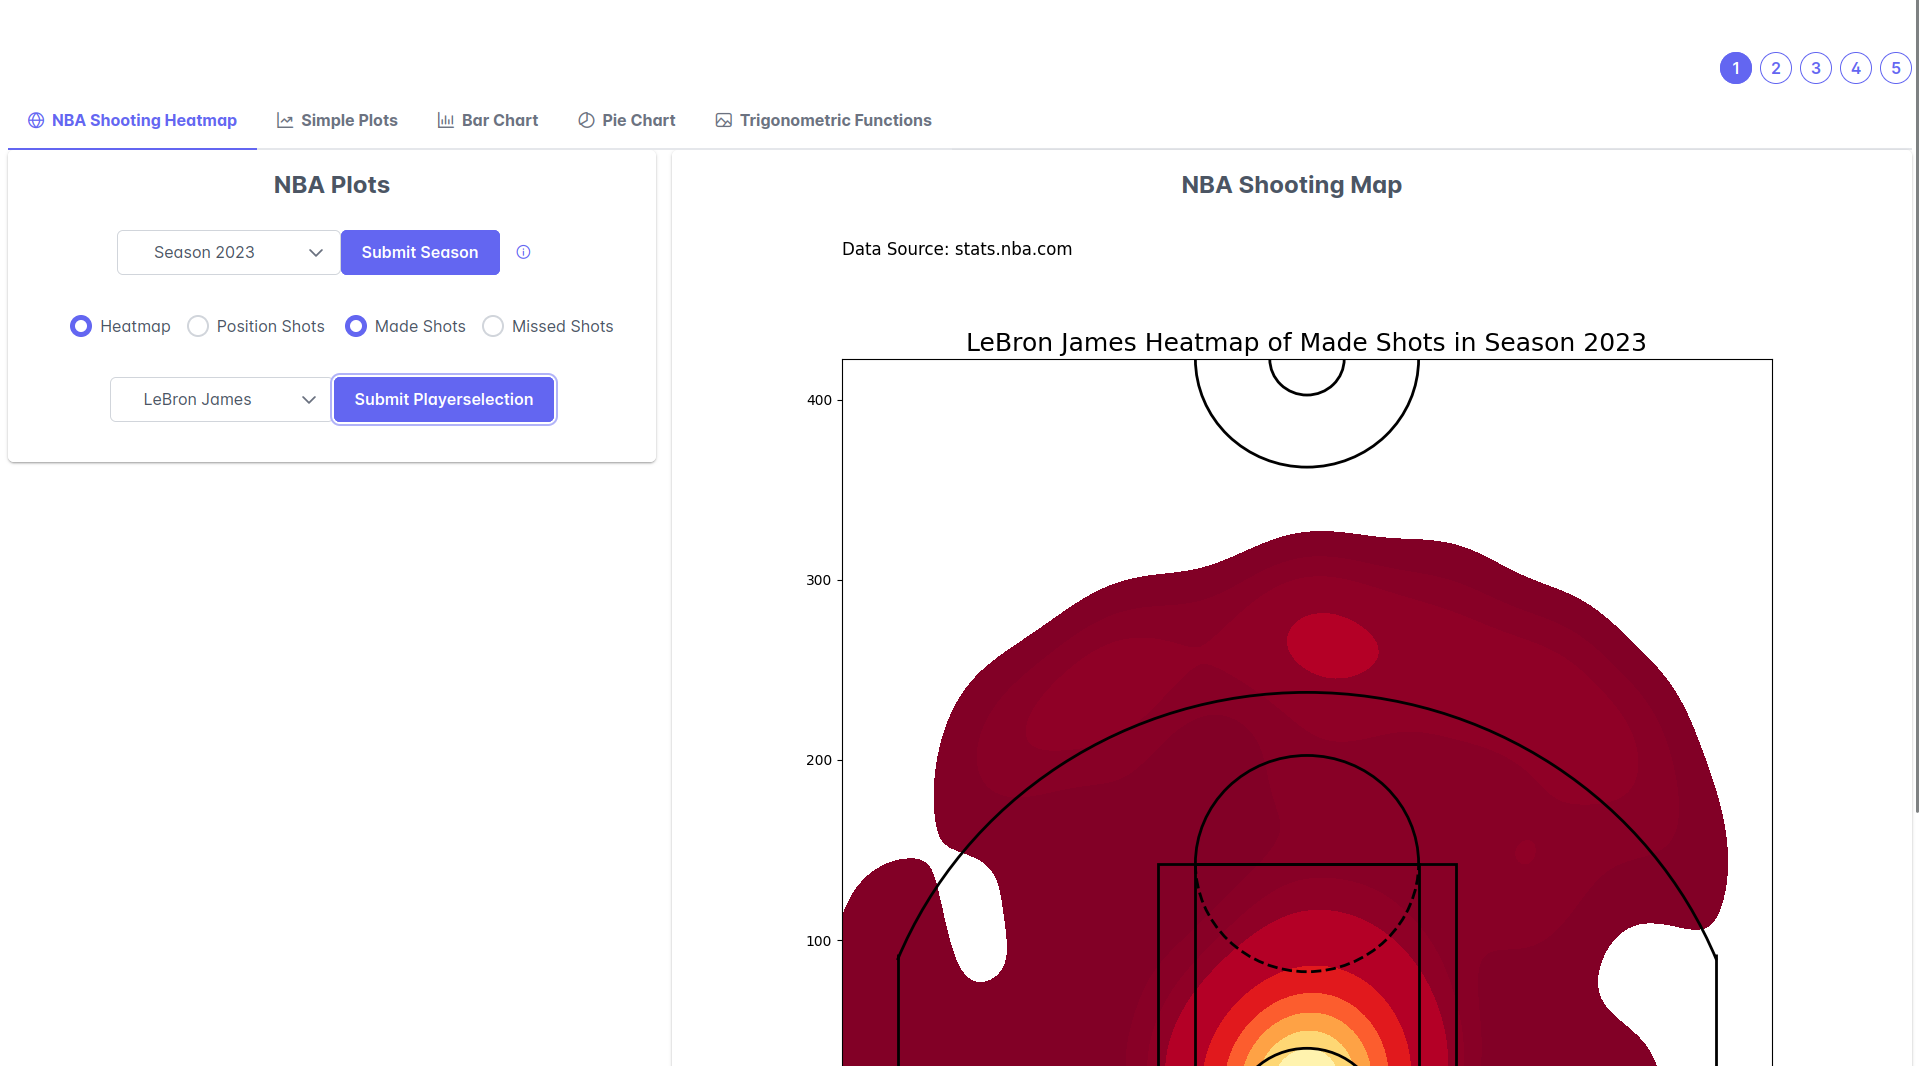
\includegraphics[width=1\textwidth]{images/NBAShooting.png}
    \caption{Option 1 view: NBA Shooting Heatmap}
    \label{fig:img1}
\end{figure}
\begin{figure}[htbp]
    \centering
    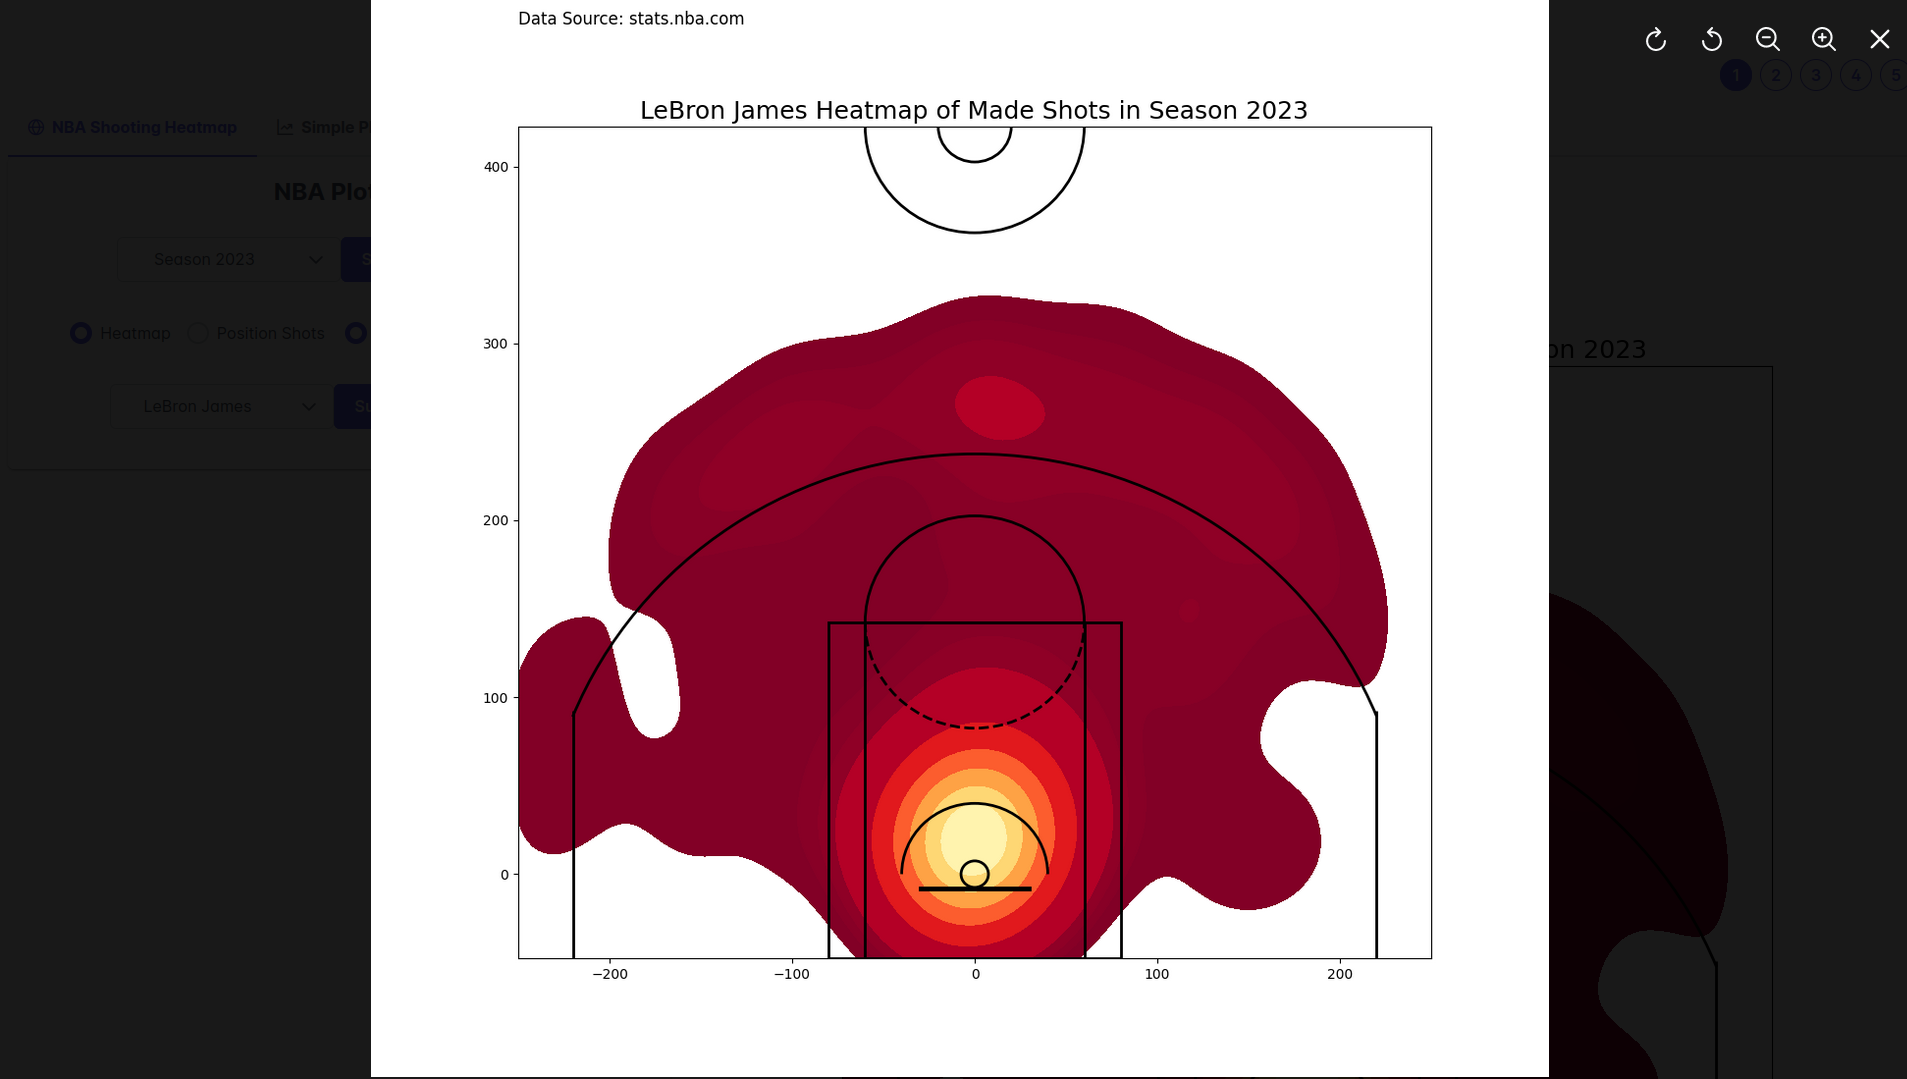
\includegraphics[width=1\textwidth]{images/imagezoomed.png}
    \caption{Images on webapp are clickable - zoomed view}
    \label{fig:img2}
\end{figure}
\begin{figure}[htbp]
    \centering
    \includegraphics[width=1\textwidth]{images/simplefunc.png}
    \caption{Option 2 view: Simple Function}
    \label{fig:img3}
\end{figure}
\begin{figure}[htbp]
    \centering
    \includegraphics[width=1\textwidth]{images/barchart.png}
    \caption{Option 3 view: Bar Charts}
    \label{fig:img4}
\end{figure}
\begin{figure}[htbp]
    \centering
    \includegraphics[width=1\textwidth]{images/piechart.png}
    \caption{Option 4 view: Pie Charts}
    \label{fig:img5}
\end{figure}
\begin{figure}[htbp]
    \centering
    \includegraphics[width=1\textwidth]{images/trigfunc.png}
    \caption{Option 5 view: Trigonometric Function}
    \label{fig:img6}
\end{figure}

\section{Conscluion}\label{sec7}

In this project, I learned a variety of skills and gained valuable experience in several areas:
\begin{itemize}
    \item \textbf{Frontend Development}: I worked with Vue.js and PrimeVue to create a user-friendly interface for interacting with a Matplotlib script.
    \item \textbf{Backend Development}: I used Flask to build the backend of my application. This involved creating routes, handling HTTP requests, and interacting with a PySQLite database to store and retrieve data.
    \item \textbf{Data Visualization}: I utilized Matplotlib, Seaborn, and other Python libraries to generate various types of plots and visualizations, such as bar charts, pie charts, heatmaps, and trigonometric plots. This involved processing data and presenting it in a visually appealing and informative way.
    \item \textbf{Dockerization}: I dockerized my application, which involved creating a Dockerfile to specify the environment and dependencies needed to run the application and using \textit{docker-compose.yml} configuration to manage two containerized services.
    \item \textbf{Project Management}: Throughout the project, I gained experience in project planning, task prioritization, and time management. In the review part, I also learned to analyze and comment on other developers codes.
\end{itemize}

Overall, this project provided me with a learning experience in web development, data visualization, database management, and containerization, equipping me with valuable skills that can be applied to future projects and in my career as a software developer.

\section{References}\label{sec10}

\begin{enumerate}
    \bibitem{flaskdocu} \href{https://flask.palletsprojects.com/en/3.0.x/quickstart/}{Flask Quickstart} - Writting A Minimal Application with Flask

    \bibitem{pysqlitedocu} \href{https://docs.python.org/3/library/sqlite3.html}{sqlite3 — DB-API 2.0 interface for SQLite databases} - A Tutorial for getting started with sqlite3.

    \bibitem{vuecli} \href{https://cli.vuejs.org/config/}{vue CLI Configuration Reference} - Guide on Global CLI Config 
    
    \bibitem{seabornkde} \href{https://seaborn.pydata.org/generated/seaborn.kdeplot.html}{seaborn.kdeplot} - Plot univariate or bivariate distributions using kernel density estimation.

    \bibitem{mathisfun} \href{https://www.mathsisfun.com/algebra/amplitude-period-frequency-phase-shift.html}{Math is Fun} - Amplitude, Period, Phase Shift and Frequency

\end{enumerate}

\bmhead{Acknowledgements} A special thanks goes out to the "Missing Semester" team, who did a very good job organizing such a practical course, where I was allowed to learn concepts that are very much used in the industry. During this course and the final project, I enhanced my knowledge a lot with interesting slides and exercises.



\begin{table}[]
\resizebox{\textwidth}{!}{%
\begin{tabular}{lp{90mm}}
Topics & \\ \hline
Liinux & Manjaro Linux is used as an operating system to test and develop the software. Other than that, there is nothing special to report. \\
Emacs & Not used. \\
VSCode & Used as a source-code editor with some extensions to improve code quality. \\
Nvim  & Nothing special to report. \\
Git & Used a Git repository to version and store code. Also used to submit the project-assignment. \\
Automation & Combined multiple technologies to automate the plotting process.  \\
Docker  & Wrote Dockerfiles and used the concept of Docker Compose for the project-assignment.  \\
Matplotlib & Used for complex plotting. \\
Gnuplot & Not used. \\
LaTex & Used to report on the project. \\
LLM's & Not used.
\end{tabular}%
}
\label{tab:proj-topics}
\end{table}
\bigskip\noindent


\bibliography{sn-bibliography}% common bib file
%% if required, the content of .bbl file can be included here once bbl is generated
%%\input sn-article.bbl


\end{document}
